\documentclass[11pt]{article}

\usepackage[top=1.1in,bottom=1.1in,left=1.2in,right=1.2in]{geometry}
\geometry{letterpaper}

\usepackage{graphicx}
\usepackage{amssymb}
\usepackage{float}
\usepackage[cmex10]{amsmath}
\numberwithin{equation}{section}

\usepackage{mathrsfs,amsthm}
\usepackage{color}
%\usepackage[scaled=.90]{helvet}

\usepackage[font=small]{caption}
\usepackage[font=footnotesize]{subcaption}


\usepackage{titlesec}
%\titleformat{\section}{\normalfont\sffamily\Large\bfseries}
%  {\thesection}{1em}{}
%\titleformat{\subsection}{\normalfont\sffamily\large\bfseries}
%  {\thesubsection}{1em}{}
%\titleformat{\subsubsection}{\normalfont\sffamily\bfseries}
%  {\thesubsubsection}{1em}{}
  
\titleformat{\section}{\normalfont\Large\bfseries}
  {\thesection}{1em}{}
\titleformat{\subsection}{\normalfont\large\bfseries}
  {\thesubsection}{1em}{}
\titleformat{\subsubsection}{\normalfont\bfseries}
  {\thesubsubsection}{1em}{}
  
  
  
% \usepackage{newtxtext}
%\usepackage{newtxmath}
\usepackage{kpfonts}
\usepackage{bm}

\usepackage{isomath}
\newcommand{\vct}{\vectorsym}
\newcommand{\mtx}{\matrixsym}

\newcommand{\lp}{\left(}
\newcommand{\rp}{\right)}

%\usepackage[sort&compress]{natbib}

\DeclareMathOperator\erf{Erf}
\DeclareMathOperator\Ei{Ei}
\DeclareMathOperator\indic{I}
\newcommand\bbR{\mathbb R}
\newcommand\bphi{\boldsymbol \phi}
\newcommand\brho{\boldsymbol \rho}
\newcommand\rect{\rm rect}
\newcommand\bx{\vct{x}}
\newcommand\by{\vct{y}}
\newcommand\ds{\boldsymbol ds}
\newcommand\bH{\boldsymbol H}
\newcommand\bF{\boldsymbol F}
\newcommand\bA{\boldsymbol A}
\newcommand\bJ{\boldsymbol J}
\newcommand\bj{\boldsymbol j}
\newcommand\bb{\boldsymbol b}
\newcommand\ba{\boldsymbol a}
\newcommand\bM{\boldsymbol M}
\newcommand\In{\operatorname{inc}}
\newcommand\Sc{\operatorname{scat}}
\newcommand\bn{\boldsymbol n}
\newcommand\br{\boldsymbol r}

\newcommand\bP{\boldsymbol P}
\newcommand\bN{\boldsymbol N}
\newcommand\bQ{\boldsymbol Q}
\newcommand\bX{\boldsymbol X}
\newcommand\bY{\boldsymbol Y}
\newcommand\bV{\boldsymbol V}
\newcommand\bu{\boldsymbol u}
\newcommand\bv{\boldsymbol v}


%%\newcommand\tot{\operatorname{tot}}
\newcommand\tot{\operatorname{}}
%\newtheorem{theorem}{Theorem}
\newtheorem{remark}{Remark}
\newtheorem{definition}{Definition}
\newtheorem{thm}{Theorem}
\newtheorem{lemma}{Lemma}

\newcommand{\cC}{\mathcal C}
\newcommand{\cT}{\mathcal T}
\newcommand{\Vo}{\mathcal V_0}
\newcommand{\To}{\mathcal T_0}
\newcommand{\Vw}{\mathcal V_\omega}
\newcommand{\Tw}{\mathcal T_\omega}

\renewcommand{\phi}{\varphi}

\title{\bf{A Fast Boundary Integral Method
    for High-Order Mesh Generation}}

%\title{\bf\sffamily A Fast Algorithm to generate smooth 
%surfaces of arbitrary shape}

\author{Felipe Vico\thanks{Instituto de Telecomunicaciones y
    Aplicaciones Multimedia (ITEAM), 
    Universidad Polit\`ecnica
    de Val\`encia, 46022 Val\`encia, Spain.
    {\em email}: {\sf felipe.vico@gmail.com,}}, \,
Leslie Greengard\thanks{Courant Institute of Mathematical Sciences,
         New York University, 
         251 Mercer Street,
         New York, NY 10012-1110.
{\em email}: {\sf greengard@cims.nyu.edu}. Research supported in
    part by ... }, \, 
and Michael O'Neil\thanks{Courant Institute of Mathematical Sciences,
         New York University, 
         251 Mercer Street,
         New York, NY 10012-1110.
{\em email}: {\sf oneil@cims.nyu.edu}. Research supported in part by
  the Office of Naval Research under award numbers
    \#N00014-17-1-2059 and \#N00014-17-1-2451.}}


\date{}



\begin{document}
\maketitle
%\tableofcontents
%\section{}
%\subsection{}




\begin{abstract}
  In this paper we present an algorithm to generate infinitely
  differentiable smooth surfaces of arbitrary shape. The surfaces can
  have arbitrary genus and multi-scale details.  The algorithm relies
  on the observation that convolution of a Gaussian in three
  dimensions with the indicator function of a closed bounded
  region~$\Omega$ generates a smooth function~$\Phi$ of three
  variables. Level sets of $\Phi$ then define infinitely smooth
  surfaces embedded in three dimensions.  With careful choices of the
  original skeleton volume~$\Omega_0$, and its skeleton surface
  mesh~$\Gamma_0$, the level set obtained via convolution is a
  \emph{smoothed} version of the original (possibly non-smooth)
  surface skeleton.  Flat regions and convexity are preserved, up to
  discretization error.  The bandlimit of the surface is locally
  controlled by the size of the skeleton mesh and the (variable) width
  of the convolving Gaussian.  The volume convolution is accelerated
  by an application of the divergence theorem and a fast multipole
  method for the resulting kernel.  We demonstrate the effectiveness
  and scaling of the algorithm using surface skeletons based on
  quadratic triangulations computed from commercial CAD and meshing
  software.  Upon completion, the resulting smooth surface is
  described by an atlas which maps the original quadratic triangles on
  the skeleton mesh to curvilinear triangles of arbitrarily high
  order.
\end{abstract}

{\bf Keywords.} High-order Surface Discretization.
Level Set. Convolution.
  Fast multipole method. Meshing algorithm.



\section{Introduction}

Integral equation methods for numerically solving many of the PDEs of
classical mathematical physics, e.g. electromagnetics, fluid dynamics,
heat flow, have come a long way over the past few decades with the
advent of fast multipole methods~\cite{}. In two dimensions, it is
often the case that near machine precision can be reached in solving
these PDEs using a modest number of unknown defined along geometries
which are known to high-order using either global parameterizations or
local piecewise-polynomial parameterizations. The associated
quadratures for the logarithmically singular Green's functions are
well-developed, and can be coupled with modern FMMs with only a modest
overhead in computational cost~\cite{qbxfmm,etc}. However, the story
is still being developed in three dimensions and most of the details
still need to be filled in.  While the three dimensional fast
algorithms (FMMs, etc.) for computing the associated $N$-body
calculations which couple with iterative solvers are well-developed,
quadratures for the weakly-singular integral operators are much a work
in progress~\cite{qbx3d,bremer,bruno}.  Even with these tools, it is
still possible to demonstrate high-order convergence and near machine
precision accuracy for solving the PDEs of mathematical
physics. However, the geometries that can be address are basically
relegated to those that are globally parameterizable:
e.g. deformations of torii and spheres.  The main roadblock to
obtaining high-order surface discretizations is the lack of meshing
algorithms which generate high-order curvilinear triangles or
quadrilateral patches.  One such software package that offers this
featuer is Gmsh~\cite{gmsh}, but in order to do so it requires, upon
input, a CAD-compatible file describing the original geometry.  In
this work, this type of tool is augmented with an algorithm which
can bootstrap low-order \emph{skeleton} meshes, such as flat
triangles, in to globally smooth high-order surfaces without the
singularities often encountered when using related methods, such as
subdivision surface generation (is this even true? there's
singularities, right?). The algorithm proposed in this work is able to
accomplish such a result by formally using a global convolution to
define a $C^\infty$ surface which can be evaluated to any fixed,
numerical precision \emph{locally}.

The existing scheme of rounding corners or two dimensional polyhedra
by Epstein and O'Neil~\cite{epsteinXXXX} can be considered the first
iteration of the algorithm in this work. In their work, the
observation was that if corners of a polygon~$\Gamma_P$ were viewed as
maps over the tangent line, convolution with a finite width
bell-function results in a smoothed curve which locally preserves
characteristics such as convexity. If the finite width bell is
replaced with a truncated Gaussian which has decayed to
size~$\epsilon$, then the resulting geometry is $C^\infty$, up to
numerically precision $\epsilon$ ({\color{red} define more specifically what we
mean here}). This entire calculation is a one-dimensional once the map
of the corner over the tangent line is calculated. Extending this
scheme, as is, to three dimensions is mathematically straightforward
but computationally and algorithmically slightly complicated by the
fact that many local maps have to be constructed wherever there are
edges or corners.

However, the scheme described above can be reformulated as a volume
convolution in which no local maps need to be constructed, only
evaluation of the indicator function of the region~$\Omega_P$ bounded
by the polygon~$\Gamma_P$. The convolution of this indicator function
with a Gaussian defined in~$\bbR^2$ defines an infinitely
differentiable function~$\Phi = \Phi(x,y)$. Furthermore, the curve
$\Gamma_{1/2}$ defined by the level set $\Phi(x,y) = 1/2$ coincides
with the boundary~$\Gamma_P$, for some suitable construction of local
maps. This scheme, volume convolution and level-set tracing, extends
directly and \emph{easily} to three dimensions, both mathematically
and computationally (assuming) that the indicator function can be
evaluated.




- need higher-order geoemtries for high order solvers (this will be
lower cost in the long run, particularly for wave propagation
problems)


The method presented here consist of finding a smooth version
$C^{\infty}$ of a given arbitrary geometry (non-smooth in general)
that we will call skeleton, where convexity, genus and flat parts are
preserved. The resulting smooth geometry has a local dependency on the
skeleton, therefore, if a small change is made at certain point of the
skeleton, the smooth surface generated by the perturbed skeleton
remains unchanged at every point except for a neighborhood of the
perturbation.




- description of skeleton

- surface discretization

- normal interpolation to get charts/watertightness

- construction of variable $\sigma$ via the fast gauss transform

- every newton step is an FMM to compute the surface to volume nodes
(in order to find the 1/2 level set)



\section{Smooth Level Sets via Convolution}



- compare with epstein/oneil



- OR for smooth surfaces, surface quadrature (fiddle with normals)



The main mathematical observation of the algorithm presented in this
work is the following: the convolution of a piecewise function, $f$
(possibly discontinuous), with a $C^\infty$ kernel, $\phi$, results in
another $C^\infty$ function, $\Phi$. This fact is of course true in any
dimension, and in particular, if we define $\indic_\Omega$ to be the
indicator function of a closed and bounded
region~$V \subset \bbR^3$ with orientable surface~$S$, then
the convolution with a kernel~$\phi$ is given by
\begin{equation}
\begin{aligned}
\Phi(\bx) &= \int_{\bbR^3} \phi(\bx-\bx') \, \indic_\Omega(\bx') \, dv(\bx') \\
 &= \int_{V} \phi(\bx-\bx')  \, dv(\bx').
\end{aligned}
\end{equation}
Clearly, in order for the above formula to be numerically useful, it
is necessary to have a method for reliably evaluating $\indic_\Omega$
and for computing integrals of truncated $\phi$'s (for integrals
crossing the bounary of~$V$). The former can be
accomplished by obtaining a surface-conforming volume mesh of the
region~$V$ and the latter requires a quadrature for smooth
functions (e.g. polynomials) on each element of the volume mesh. The
level sets of~$\Phi$, $\Phi(\bx) = C$, then define smooth
surfaces~$\Gamma_C$ embedded in~$\bbR^3$.

If~$\phi$ is compactly supported and $\int \phi = 1$ then flat regions
of~$S$ which extend beyond the range of~$\phi$ are preserved
along the~$\Phi = 1/2$ level set. This can easily be shown in the
one-dimensional case~\cite{epstein_2016} and is straightforward so
show in higher dimensions. Furthermore, for compactly supported~$\phi$
the above convolution is a completely local calculation, and therefore
has optimal asymptotic computational scaling regardless of the
implementation. However, there is of course a tradeoff: kernels with
narrow support preserve small features of the domain~$\Omega$ and its
boundary~$\Gamma$, and therefore may produce areas of high
curvature. Convolution with significantly wider kernels require a
significant increase in computational cost over the narrow case.

Furthermore, the above volume integral can be reformulated as a
boundary integral via an application of the divergence
theorem. If~$\phi$ can be chosen as an exact
function,~$\phi = \nabla \cdot \vct{F}$, for some
vectorfield~$\vct{F}$, then we have that:
\begin{equation}
  \begin{aligned}
    \Phi(\bx) &= \int_{V} \nabla \cdot \vct{F}(\bx-\bx') \, dv(\bx') \\
    &= \int_{S} \bn(\bx') \cdot \vct{F}(\bx-\bx') \, da(\bx')
  \end{aligned}
\end{equation}
where~$\bn(\bx')$ is the outward unit normal to the surface~$S$ at the
point~$\bx'$. The above formula will turn out to be useful in
designing a fast algorithm, but we will put it aside for now as it is
equivalent to the volume calculation. We now turn to computing an
atlas (i.e. a collection of parameterizations) describing the
convolution surface~$\Gamma_C$.





\subsection{Constructing an Atlas}

In what follows, the boundary~$S$ of the original volume~$V$ will be
referred to as the \emph{skeleton surface}. Often~$S$ will be supplied
as a low-order mesh (e.g. flat triangles), and will be assumed to be
water-tight and oriented (i.e. have a consistent collection of normal
vectors). The construction of the atlas will be described assuming an
initial collection of flat skeleton triangles, but is straightforward
to extend to other configurations (e.g. quadratic triangles, flat
quadrilaterals, etc.). To this end, the skeleton surface~$S$ is the
union of~$M$ triangles~$T^j$, $j=1,\ldots,M$, with each triangle
having vertices denoted
by~$\{ \vct{P}^j_1,\vct{P}^j_2,\vct{P}^j_3 \} $.
Therefore, each skeleton triangle is parameterized as:
\begin{equation}
  \vct{T}^j(u,v) = \vct{P}^j_1 + u \lp \vct{P}^j_2 - \vct{P}^j_1 \rp
  + v \lp \vct{P}^j_3 - \vct{P}^j_1 \rp,
\end{equation}
and has Frenet basis defined by
\begin{equation}
\vct{T}^j_u = \frac{\vct{P}^j_2 - \vct{P}^j_1}{\left| \vct{P}^j_2 -
    \vct{P}^j_1 \right|}, \qquad
\vct{T}^j_v = \frac{\vct{P}^j_3 - \vct{P}^j_1}{\left| \vct{P}^j_3 -
    \vct{P}^j_1 \right|}, \qquad
\vct{N}^j =  \vct{T}^j_u \times \vct{T}^j_v.
\end{equation}
Despite the assumption of water-tightness on the skeleton mesh, the
normal vectors are obviously discontinuous across triangle edges. The
following construction of an atlas will be based on a mapping of each
skeleton triangle to a high-order curvilinear one along the
surface~$\Gamma_{1/2}$. In order to define a unique \emph{mapping
  direction} (since vectors along the normal direction will intersect
at arbitrarily close locations to the skeleton mesh), we define the
vectorfield~$\vct{H}$ along the surface to be a local averaging of the
unit normal vectors. We begin by defining~$\vct{H}$ at each of the
vertices.  First, denote the list of triangles for
which~$\vct{P}^j_\ell$ is a common vertex by~$\cT \vct{P}^j_\ell$,
\begin{equation}
  \cT \vct{P}^j_\ell = \left\{ i \text{ such that } T^i \text{
      contains } \vct{P}^j_\ell \right\}.
\end{equation}
The value of the vectorfield~$\vct{H}$ at the vertex~$\vct{P}^j_\ell$
is then set to be
\begin{equation}
  \vct{H}^j_\ell = \frac{1}{
    \left|  \cT \vct{P}^j_\ell \right| } \sum_{i \in \cT
    \vct{P}^j_\ell} \vct{N}^i.
\end{equation}
The above is merely a local averaging of the normal vectors associated
with each triangle that shares~$\vct{P}^j_\ell$, and the
vector~$\vct{H}^j_\ell$ will be referred to as the \emph{vertex normal}
at~$\vct{P}^j_\ell$. This construction extends straightforwardly to
various other skeleton patches; the vertex normal can, in general, be
defined as some weighted average of the normals of the adjacent triangles.
See Figure~\ref{normalvert1}. {\color{red} Update notation in Figure.}

\begin{figure}[t]
  \centering
  \begin{subfigure}[b]{.3\linewidth}
    \centering
    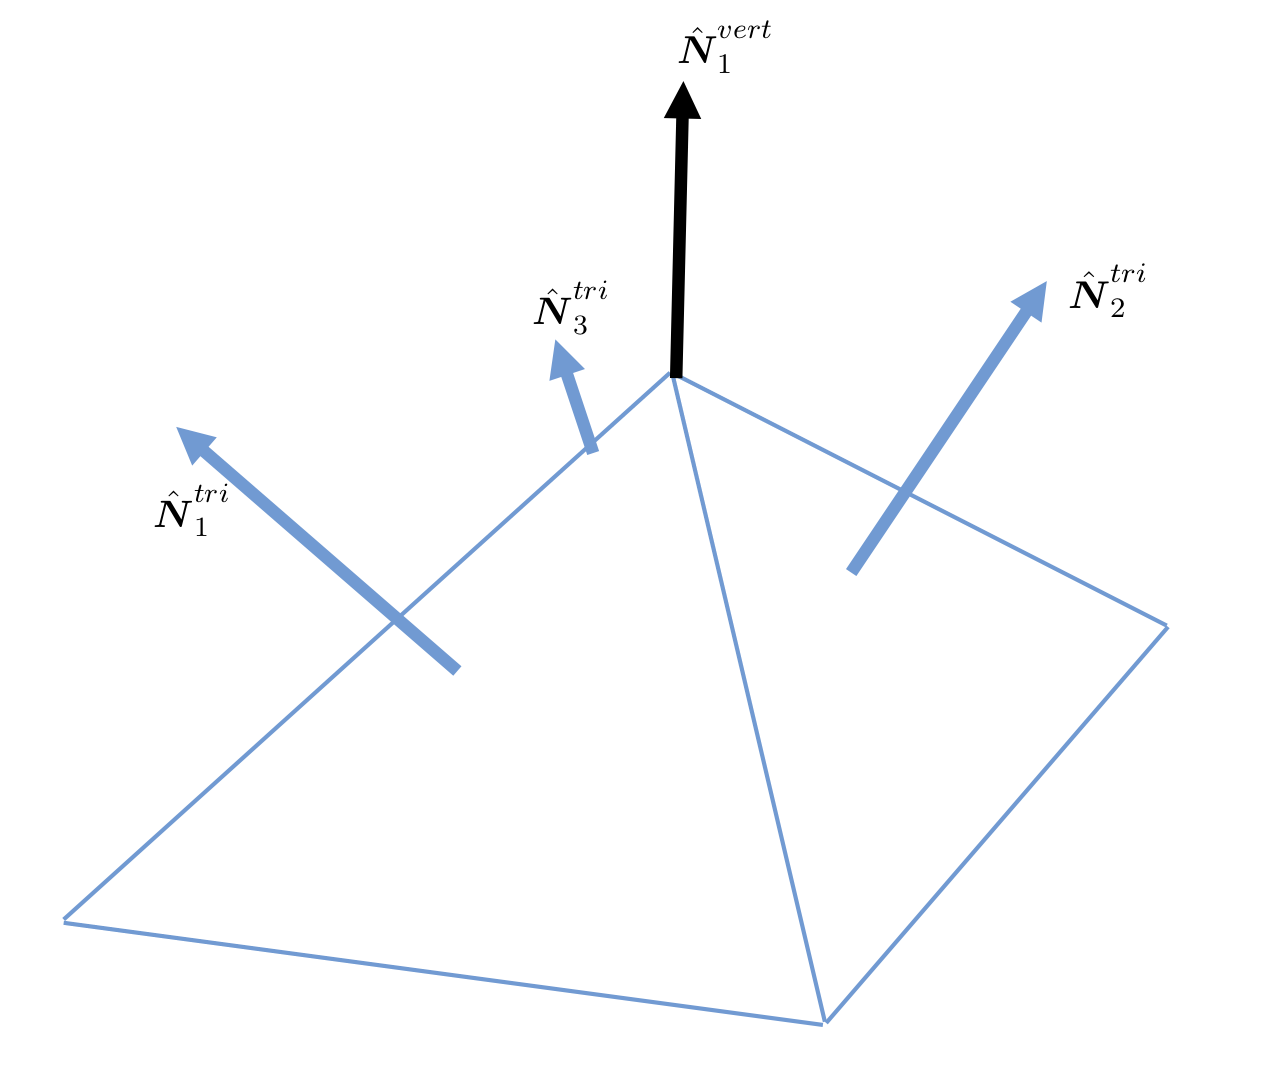
\includegraphics[width=\linewidth]{normal_vertex.png}%
    \caption{Vertex normal vector.}
    \label{normalvert1}
  \end{subfigure}
  \hfill
  \begin{subfigure}[b]{.3\linewidth}
    \centering
    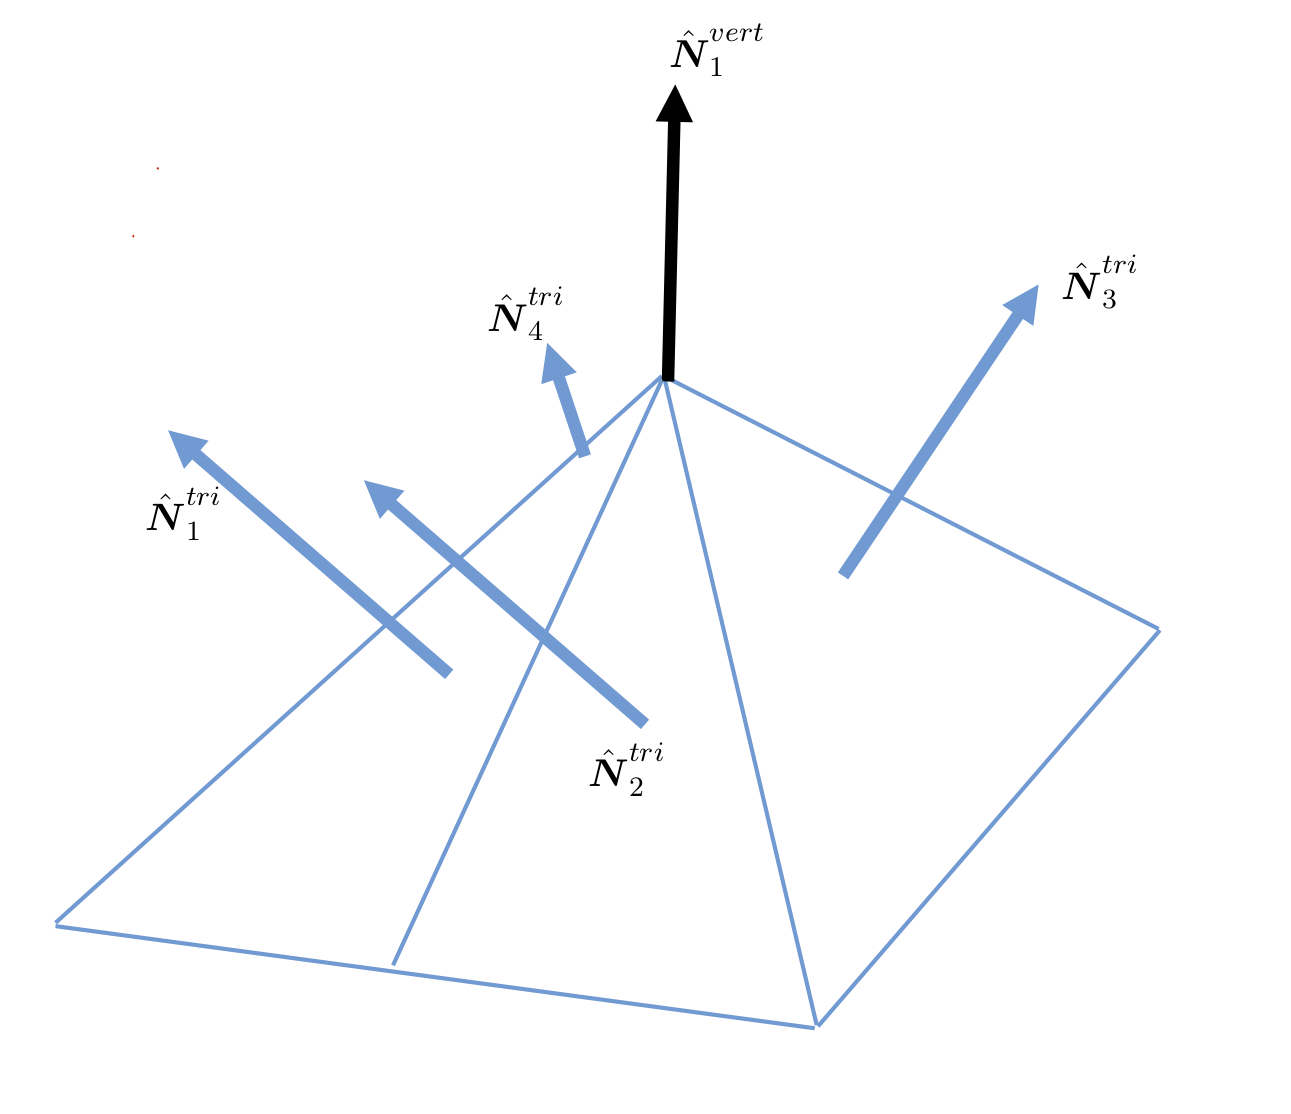
\includegraphics[width=\linewidth]{normal_vertex_2.png}%
    \caption{Weighted vertex normal.}
    \label{normalvert2}
  \end{subfigure}
  \hfill
  \begin{subfigure}[b]{.3\linewidth}
    \centering
    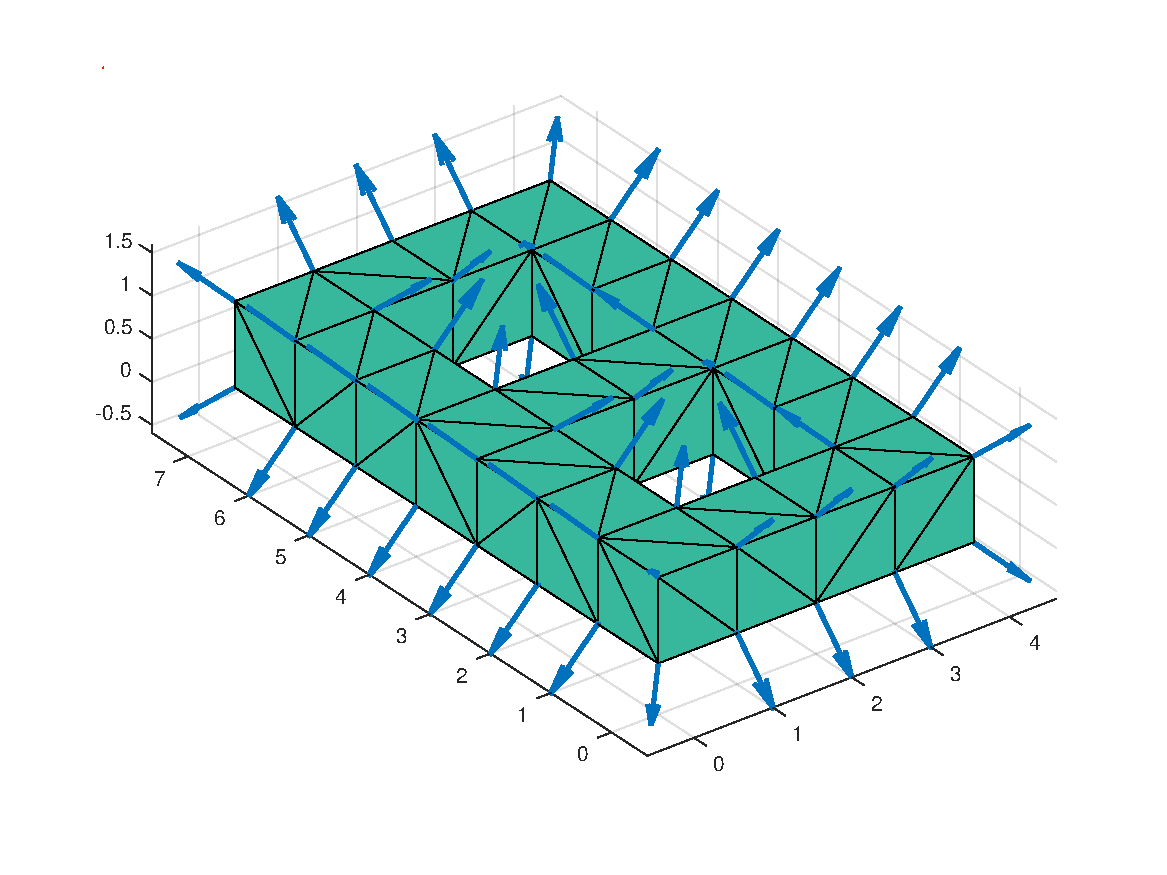
\includegraphics[width=\linewidth]{normal_vert_genus_2.pdf}%
    \caption{Skeleton and vertex normals.}
    \label{normalvert3}
  \end{subfigure}
  
  \caption{Construction of the vertex normals.}
  \label{fig:normalverts}
\end{figure}




One such reasonable choice of weighting is that of what we will refer
to as \emph{vertex angle}, not to be confused with the more commonly
used dihedral angle in geometry. The vertex angle of triangle~$T^j$
at vertex~$\vct{P}^j_\ell$ is merely the interior angle of the
triangle at this vertex. Depending on the order of the vertex, the
total sum of all vertex angles of all adjacent triangles will be
different; denote by $\theta^j_\ell$ the vertex angle of
triangle~$T^j$ at vertex~$\vct{P}^j_\ell$ and the total vertex angle
(sum of all vertex angles) by~$A^j_\ell$. The vertex normals can then
be computed using the vertex angle weighting as
\begin{equation}
  \vct{H}^j_\ell = \frac{1}{ A^j_\ell} \, 
  \sum_{i \in \cT \vct{P}^j_\ell} 
  \theta^j_\ell \,  \vct{N}^i.
\end{equation}
See Figure~\ref{normalvert2}.
Along the interior of skeleton triangle~$T^j$, the
vectorfield~$\vct{H}$ is extended via convex combination:
\begin{equation}
  \vct{H}^j(u,v) = \vct{H}^j_1 + u \lp \vct{H}^j_2 - \vct{H}^j_1 \rp
  + v \lp \vct{H}^j_3 - \vct{H}^j_1 \rp.
\end{equation}
Note that this vectorfield is now continuous across the edges of each
skeleton triangle. See Figure~\ref{normalvert3}.

The convolution surface~$\Gamma_C$ (i.e. the level-set $\Phi = C$)
will be parameterized piecewise above/below each skeleton triangle as
\begin{equation}\label{eq:h}
  \vct{x}^j(u,v) = \vct{T}^j(u,v) + h^j(u,v) \, \vct{H}^j(u,v),
\end{equation}
with $\vct{x}^j$ denoting the chart which generates the patch~$\Gamma^j_C$
from the skeleton mesh. The function~$h^j$ can be determined
pointwise as the solution to the equation
\begin{equation}\label{eq:newton}
  \Phi\lp \vct{x}^j(u,v)  \rp - C = 0.
\end{equation}
The above is still an implicit definition of the surface, but for a
particular location~$(u,v)$ in parameter space, it can be solved
for~$h(u,v)$ relatively easily using Newton's method, assuming that
the~$\Phi$ can be easily evaluated. Newton's method also requires the
evaluation of the derivative of~$\Phi$, which in this case can be
computed as
\begin{equation}
  \begin{aligned}
  \frac{\partial \Phi}{\partial h} &= \frac{\partial }{\partial h}
  \int_V \phi\lp \vct{T} + h\, \vct{H} - \bx'\rp \, da(\vct{x}') \\
  &= \int_V \vct{H} \cdot \nabla \phi\lp
  \vct{T} + h\, \vct{H} - \bx'\rp \, da(\vct{x}'),
\end{aligned}
\end{equation}
where we have suppressed the dependence on the patch~$j$.  The final
surface is obtained piecewise by the collection of chartss~$\vct{x}^j$.
Each chart~$\vct{x}^j:T_0 \to \bbR^3$ is smooth, and inherits the
regularity properties of the convolution kernel~$\phi$. Here,~$T_0$
denotes the standard simplex triangle $0 \leq u+v \leq 1$ with
$u,v >0$.



\begin{figure}[t]
  \centering
  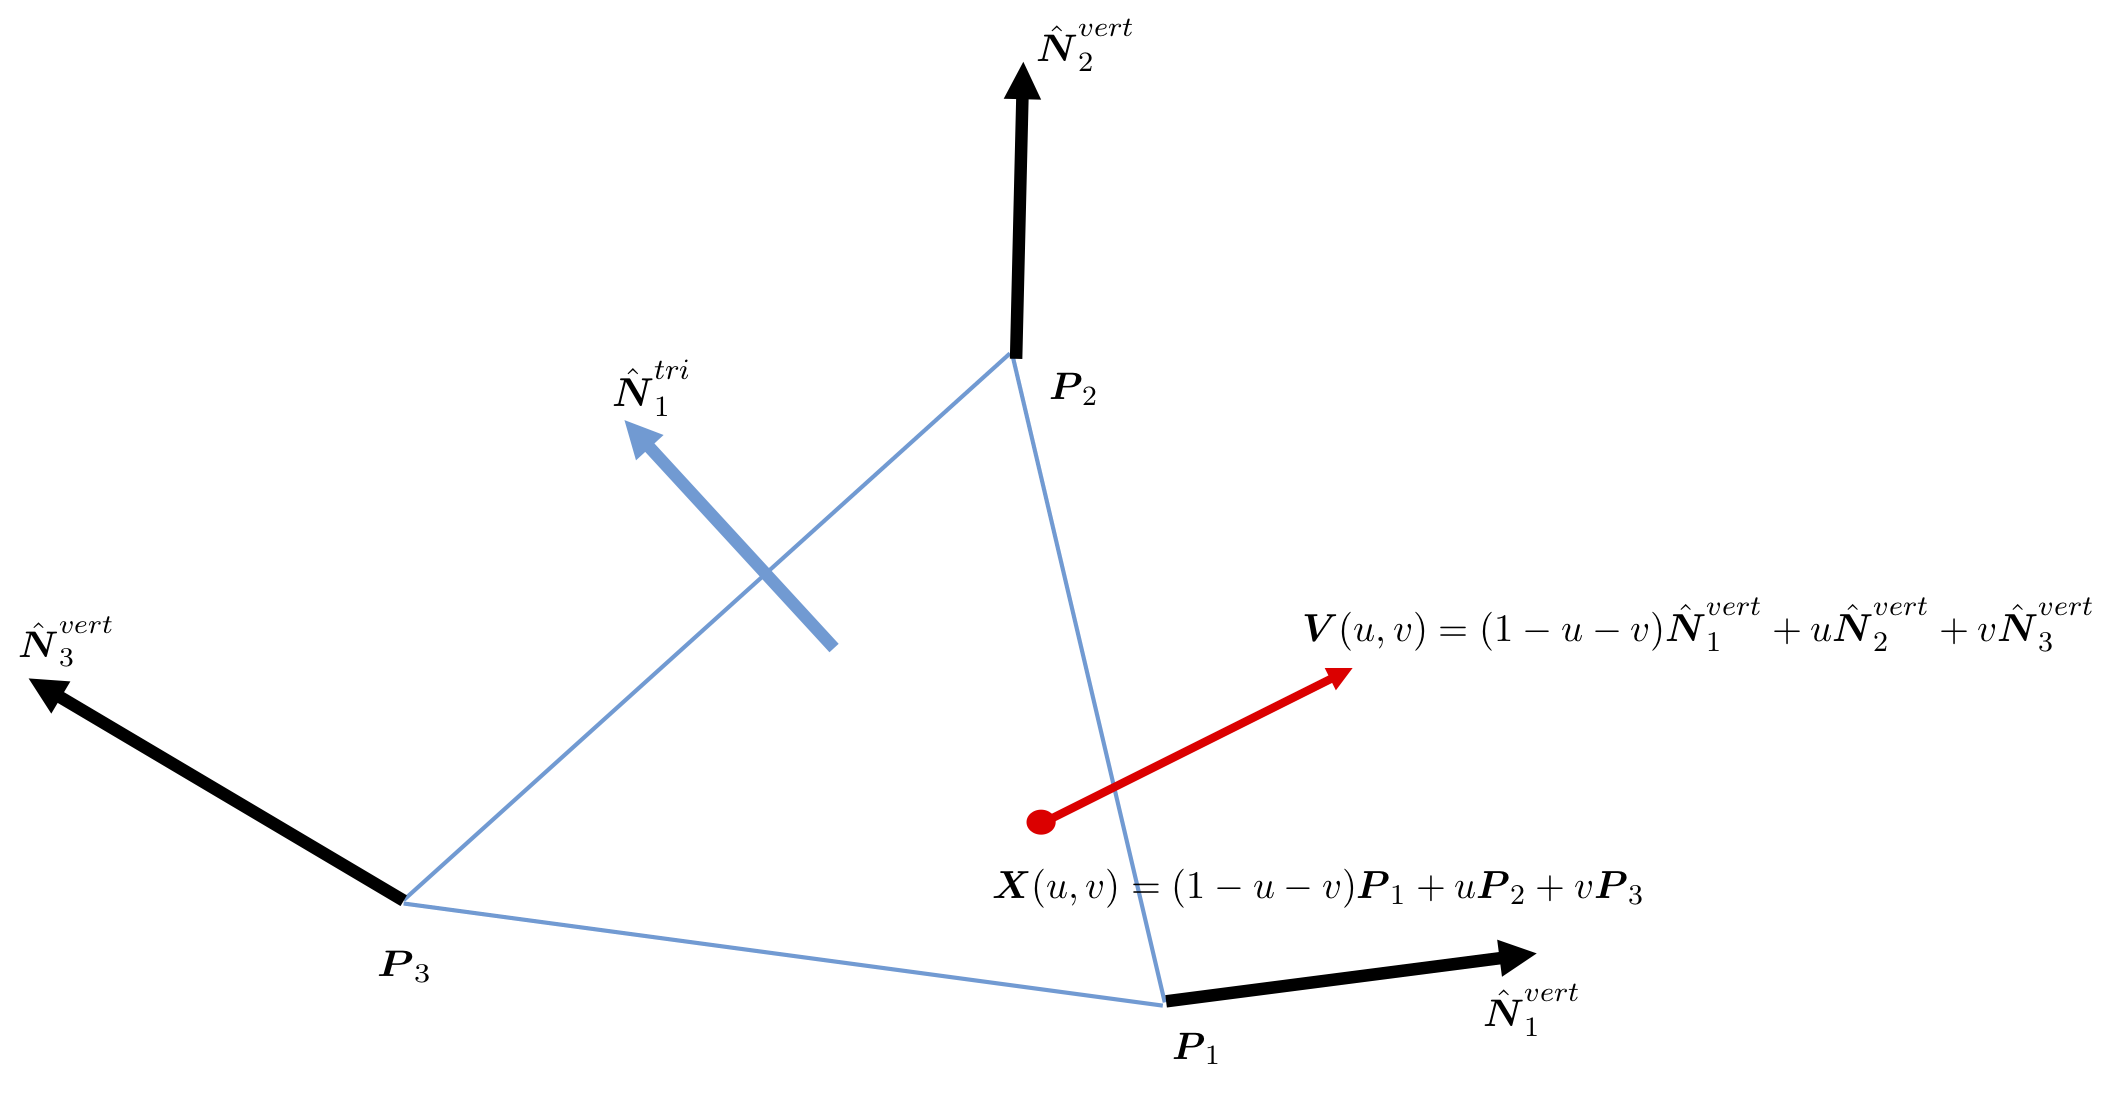
\includegraphics[width=.65\linewidth]{normal_vertex_3.png}%
  \caption{The interpolated value of the vertex normal to the interior
    of the triangle.}
  \label{normalvert3}
\end{figure}




% Let's consider a Gaussian function of 3 variables:
% $k(\bx)=\frac{1}{\sigma^3\sqrt{2\pi}^3}e^{-\frac{r^2}{2\sigma^2}}$,
% where $r=|\bx|$ and $\bx\subset \mathbb{R}^3$. For the moment we will
% consider $\sigma$ as a constant.  Let's define the convolution of the
% indicator function on $\mathit{V}$ and the Gaussian:
% $$f(\bx)=\int_{V}k(\bx-\by)dV_{\by}$$
% Now we define the surface $\mathcal{S}=\{\bx \mid f(\bx)=\frac{1}{2}\}$.

% For a suitable selection of the parameter $\sigma$ (small enough), the
% resulting surface $\mathcal{S}$ is a smooth version of $\mathit{S}$,
% of class $C^{\infty}$. Notice also that we can control the degree of
% smoothness obtained by changing the value of the parameter
% $\sigma$. For $\sigma \rightarrow 0$, the surface obtained converges
% to the original skeleton $\mathcal{S}\rightarrow \mathit{S}$.

% Notice also that we can generalize this process to any skeleton
% $\mathit{S}$ (not only triangulated surfaces), and the same regularity
% on $\mathcal{S}$ will be obtained.








\subsection{Local Coordinates}

In this section we find suitable expressions to obtain a local
orthonormal basis along each patch of the surface~$\Gamma^j$, as well
as the area element.
Recall that the chart for the patch~$\Gamma^j$ is given by
\begin{equation}\label{chart}
    \vct{x}^j(u,v) = \vct{T}^j(u,v) + h^j(u,v) \, \vct{H}^j(u,v).
\end{equation}
Taking the partial derivative with respect to~$u$ above, we have
\begin{equation}\label{u_vector}
  \begin{aligned}
    \vct{x}^j_u(u,v) &=  \frac{\partial \vct{x}^j}{\partial u}(u,v) \\
    &= \vct{T}^j_u + h(u,v) \,
  \vct{H}^j_u   + \frac{\partial h}{\partial
    u}(u,v)
  \, \vct{H}^j(u,v).
  \end{aligned}
\end{equation}
where the only unknown term is~$\partial h / \partial u$ (since it was
only~$h$ that was computed via Newton's algorithm, as in the previous
section).
However, using the fact that~$\partial\vct{x}^j/\partial u$ must be
tangent to the surface~$\Gamma_C$, and that~$\nabla \Phi$ is normal
to~$\Gamma$ (easily shown from computation), we have
\begin{equation}\label{U_vector_2}
  \frac{\partial h}{\partial u} = \frac{\lp \vct{T}^j_u + h \, \vct{H}^j_u
  \rp \cdot \nabla \Phi }{\vct{H}^j \cdot \nabla \Phi}.
\end{equation}
A similar calculation can be used to obtain
\begin{equation}\label{v_vector}
    \vct{x}^j_v
    = \vct{T}^j_v + h \,
  \vct{H}^j_v   + \frac{\partial h}{\partial
    v}
  \, \vct{H}^j
\end{equation}
with
\begin{equation}\label{v_vector_2}
  \frac{\partial h}{\partial v} = \frac{\lp \vct{T}^j_v + h \, \vct{H}^j_v
  \rp \cdot \nabla \Phi }{\vct{H}^j \cdot \nabla \Phi}.
\end{equation}
{\color{red} fix length scaling of chart to be consistent with
  evarythign else, either normalize or don't}



now we can write the area element $dS$ as:

\begin{equation}\label{dS}
\begin{aligned}
 dS=\Bigg|\frac{\partial\bY(u,v)}{\partial u}\times\frac{\partial\bY(u,v)}{\partial v}\Bigg|dudv
\end{aligned}
\end{equation}
  
%therefore:
 
% $$W_n=\Bigg|\frac{\partial\bY}{\partial u}(u_n,v_n)\times\frac{\partial\bY}{\partial v}(u_n,v_n)\Bigg|w_n$$
 
As tangent reference system on the surface we use the vectors $\hat{\bu}, \hat{\bv}$; for the  $\hat{\bu}$ vector we normalize $\frac{\partial\bY(u,v)}{\partial u}$, and for the $\hat{\bv}$ vector we cross $\frac{\nabla f}{|\nabla f|}$ with $\hat{\bu}$.





We now turn to describing a fast adaptive high-order algorithm for
numerically approximating the surface~$\Gamma_C$, as constructed
above, that is compatible with many boundary integral equation
discretization schemes.








\section{A Fast Algorithm}
\label{sec:algorithm}

The previous discussion has taken place without any numerical
considerations. In order to make the scheme as described a viable
numerical method, several elements have to be made computationally
tractable: for example, numerical evaluation of ~$\Phi$ (a volume
integral), approximation/discretization of the surface~$\Gamma_C$, and
implementation of Newton's method to determine the function~$h$
in~\eqref{eq:h}.
We begin by reformulating the expression for~$\Phi$ in terms of a
boundary integral, thereby obviating the need to mesh the interior
volume of the region~$V$.


\subsection{Boundary Integral Formulation}
\label{sec:bif}

Until this point, the convolution kernel~$\phi$ has not been
specified, aside from suggestions that certain advantages come from it
being compactly supported. In applications such as this, where
convolution is being used as a method to generate what we could call a
\emph{bandlimited surface}, there are two natural choices: a Gaussian
and the Kaiser-Bessel window~\cite{barnett2018}. In this work we
choose to use a Gaussian as the convolution kernel for various
reasons, namely for the ease with which the divergence theorem can be
applied to the volume convolution. The following identity allows us to
directly represent~$\Phi$ as a boundary integral: 
\begin{equation}
  \Delta \lp \frac{1}{4\pi r} \erf \lp \frac{r}{\sqrt{2}\sigma} \rp
  \rp = - \frac{1}{\lp 2\pi \sigma^2 \rp^{3/2}} e^{-r^2/2\sigma^2}.
\end{equation}
where~$\erf$ is defined to be an integral of the Gaussian:
\begin{equation}
\erf(r) = \frac{2}{\sqrt{\pi}} \int^r_0 e^{-t^2} \, dt.
\end{equation}
Using the above identity, we can rewrite~$\Phi$ as
\begin{equation}\label{eq:surf}
  \begin{aligned}
    \Phi(\vct{x}) &= \int_V \frac{1}{\lp 2\pi \sigma^2 \rp^{3/2}}
    e^{-|\vct{x}-\vct{x}'|^2/2\sigma^2} \, dv(\vct{x}') \\
    &= - \int_V \Delta \lp \frac{1}{4\pi |\vct{x}-\vct{x}'|}
    \erf \lp \frac{|\vct{x} - \vct{x}'|}{\sqrt{2}\sigma} \rp
    \rp \, dv(\vct{x}') \\
    &= - \int_S \vct{N}(\bx) \cdot \nabla_{\vct{x}}
     \lp \frac{1}{4\pi |\vct{x}-\vct{x}'|}
    \erf \lp \frac{|\vct{x} - \vct{x}'|}{\sqrt{2}\sigma} \rp
    \rp \, ds(\vct{x}') \\
    &=\int_S  \vct{N}(\vct{x}) \cdot \lp \vct{x} -\vct{x}' \rp \lp
    \frac{\erf \lp |\bx-\bx'|/ \sqrt{2}\sigma \rp
    }{4\pi|\bx-\bx'|^3}
    -\frac{\sqrt{\frac{2}{\pi}}e^{-|\bx-\bx'|^2/2\sigma^2}}{4\pi\sigma|\by-\bx|^2}
    \rp \, da(\bx') \\
    &= \int_S \psi(\bx-\bx') \, da(\bx').
  \end{aligned}
\end{equation}
Note that the kernel in the above surface integral, denoted by~$\psi$,
is smooth. Furthermore, for even modestly large values of~$r$, we have
that
\begin{equation}
  \erf(r) \approx 1, \qquad e^{-r^2} \approx 0.
\end{equation}
This means that in the far-field we can approximate the kernel~$\psi$ as
\begin{equation}
  \psi(\bx-\bx') \approx -\vct{N}(\bx) \cdot \nabla_{\bx} \left(
    \frac{1}{4\pi |\bx-\bx'| }\right).
\end{equation}
The above approximation is the same as the kernel appearing in
double-layer potentials when solving Laplace's equation in three
dimensions using integral equation methods. This type of kernel admits
very efficient, asymptotically optimal~$n$-body summations via fast
multipole methods~\cite{many}, and therefore the resulting boundary
integral in~\eqref{eq:surf} can be applied efficiently.
For a given target location~$\bx$, the surface integral above can be
split into two pieces:
\begin{equation}
  \Phi(\bx) = \int_{S\setminus B(\bx,R)} \vct{N}(\bx) \cdot \nabla_{\bx} \left(
    \frac{1}{4\pi |\bx-\bx'| }\right) \, da(\bx') +
  \int_{S \cap B(\bx,R)} \psi(\bx-\bx') \, da(\bx'),
\end{equation}
where~$R$ is chosen such that~$\Phi(\bx)$ is computed to some
specified accuracy~$\epsilon$. The first term above (the far-field)
can be discretized and computed using an FMM for Laplace potentials;
the second term can be discretized using quadratures for smooth
functions and computed directly, without the aid of any fast algorithm.
It easy to check that the gradient of the above expression can also be
efficiently evaluated using an FMM, as the gradient of the far-field
term is also a Laplace potential. The gradient can be expanded as:
\begin{equation}\label{eq:surfgrad}
    \nabla \Phi(\bx) =  ...
\end{equation}
{\color{red} Sign check and insert correct formula above.}
% \begin{equation}\label{surf_nablaf}
% \begin{aligned}
%   \nabla f(\bx)&=\int_{\mathit{S}}\nabla_{\bx}\nabla_{\by}\Big(\frac{\erf\big(\frac{|\by-\bx|}{\sqrt{2}\sigma}\big)}{4\pi|\by-\bx|}\Big)\cdot\bn(\by)dS_{\by}=\\
%   &=\int_{\mathit{S}}-\bn(\by)\Bigg(\frac{\erf\big(\frac{|\by-\bx|}{\sqrt{2}\sigma}\big)}{4\pi|\by-\bx|^3}-\frac{\sqrt{\frac{2}{\pi}}e^{-\frac{|\by-\bx|^2}{2\sigma^2}}}{4\pi\sigma|\by-\bx|^2}\Bigg)dS_{\by}+\\
%   +&\int_{\mathit{S}}
%   -\frac{e^{-\frac{r^2}{2\sigma^2}}(\sqrt{2}r^3+\sqrt{2}r\sigma^23)-\sigma^3\sqrt{\pi}3\erf{\big(\frac{r}{\sqrt{2}\sigma}}\big)}{r^5\sigma^3\pi^{3/2}4}(\bx-\by)<(\by-\bx)\cdot
%   \hat{\bn}(\by)>dS_{\by}
% \end{aligned}
% \end{equation}
%where $r=|\bx-\by|$. In this case we also have that, for far distances
%between source and target, we can approximate the kernel by:

% \begin{equation}
% \begin{aligned}
%   \nabla_{\bx}\nabla_{\by}\Big(\frac{\erf\big(\frac{|\by-\bx|}
% {\sqrt{2}\sigma}\big)}{4\pi|\by-\bx|}\Big)\cdot\bn(\by)\approx
%   \nabla_{\bx}\nabla_{\by}\Big(\frac{1}{4\pi|\by-\bx|}\Big)\cdot\bn(\by)
% \end{aligned}
% \end{equation}

% Which is the kernel of the gradient of the double layer with density
% $=1$, therefore we can use again the FMM to compute it. For the near
% interaction, the kernel is again smooth.

With the above reformulation of the evaluation of~$\Phi$ as a boundary
integral, and its calculation accelerated via an FMM, this means that
the Newton iteration for determining~$h$ in~\eqref{eq:newton} can be
performed \emph{simultaneously for every discretization point along
  $S$}. We now turn to the actual high-order approximation of the
smoothed surface, which will involve using a high-order quadrature
along the skeleton mesh and approximation using orthogonal polynomials
on the simplex.




\subsection{High-Order Discretization}
\label{sec:disc}

In this section we describe a method for discretizing the surface
integral appearing in~\eqref{eq:surf} and subsequently approximating
the convolution surface~$\Gamma_C$ using a piecewise polynomial
approximation over the standard simplex triangle. Under our
assumption, the skeleton surface is provided as a collection of flat
triangles. In order to evaluate the boundary integral over this
surface with kernel~$\psi$, we discretize the integral on each
triangle using what are known as Vioreanu-Rokhlin
quadratures~\cite{vioreanu_2014}. These quadrature rules are very
efficient and are \emph{Gaussian-like} in that they integrate more
functions than there are nodes in the quadrature. The actual order of
the quadrature varies with the order of the underling implied
interpolation, see~\cite{vioreanu_2014} for details.
On the simplex~$T_0$, we
denote a polynomial of degree~$q$ in two variables as
\begin{equation}
  f(u,v) = \sum_{m+n \leq q} a_{mn} \, u^m \, v^n.
\end{equation}
The polynomial~$f$ above is said to be of order~$q$ and its expansion
has~$(q+1)(q+2)/2$ linearly independent polynomials. Since 



considered a nextension of Gaussian quadrature to the triangle, as
they 


propose a fast algorithm to discretize the surface
to high order. As a result we will obtain, for each triangle
$\mathcal{T}_j$, a set of points $(\bY_n=\bY(u_n,v_n))_{n=1}^N$ where
$(u_n,v_n)_{n=1}^N$ are the nodes associated to a generalized Gaussian
quadrature rule for smooth functions on the canonical triangle (see
[Rokhlin Gaussian Smooth Triangle]). As a result, we will also obtain
tangent and norlam vectors associated to each point
$\hat{\bu}_n,\hat{\bv}_n,\hat{\bn}_n$, and a weight $dS_n$ to compute
surface integrals of smooth functions on the surface to high order.

Let's consider a particular high order generalized Gaussian rule on
the canonical triangle $(u_n,v_n,w_n)_{n=1}^N$, where $u_n,v_n$ are
nodes and $w_n$ are weights. For each triangle $\mathcal{T}_j$ and
each node $u_n,v_n$ we consider the equation of one variable $h$:

\begin{equation}\label{newtoneq}
f(\bX(u_n,v_n)+\bV(u_n,v_n)h)=\frac{1}{2}
\end{equation}

We run the Newton's method to find the root. In order to do that we need a fast method to compute both $f$ and $\nabla f$. Next section is about a fast algorithm to compute it.

Notice that the value of $h$ depends on $u_n,v_n$, therefore we can write $h(u_n,v_n)$. Once this value is found, we can obtain the tangent and normal vectors to the surface at those points $\bY_n$ by evaluating the expressions \ref{U_vector}, \ref{U_vector_2} and \ref{V_vector} and \ref{V_vector_2}. We can also obtain the weights using \ref{dS} as:

\begin{equation}\label{dS_n}
\begin{aligned}
 W_n=\Bigg|\frac{\partial\bY(u_n,v_n)}{\partial u}\times\frac{\partial\bY(u_n,v_n)}{\partial v}\Bigg|w_n
\end{aligned}
\end{equation}

Finally, we obtain the orthogonal system at each discretization point as:

\begin{equation}
\begin{aligned}
\bn_n=\frac{\nabla f(\bY_n)}{|\nabla f(\bY_n)|},\  \  \  \   \ 
\bu_n=\frac{\frac{\partial\bY(u_n,v_n)}{\partial u}}{|\frac{\partial\bY(u_n,v_n)}{\partial u}|},\  \  \  \   \
\bv_n=\bn_n\times\bu_n
\end{aligned}
\end{equation}




\subsection{Refinement}

In this section we describe the process to obtain a refined version of the discretization. The process consist of splitting each curved triangle  $\mathcal{T}_j$ of the original chart into four triangles, and then apply the discretization process described in section \ref{disc} to each sub-triangle.

Each chart of $\mathcal{T}_j$ can be written as:

\begin{equation}
\bY(u,v)=\bX(u,v)+\bV(u,v)h(u,v)
\end{equation}

For $(u,v)$ in the unitary triangle $0\le u, 0\le v, u+v\le1$ and $h(u,v)$ verifying the equation:

\begin{equation}
f(\bX(u,v)+\bV(u,v)h(u,v))=\frac{1}{2}
\end{equation}

Now we consider four subdomains of the unitary triangle as shown in the figure \ref{refinement1}:

\begin{figure}[H]
\begin{center}
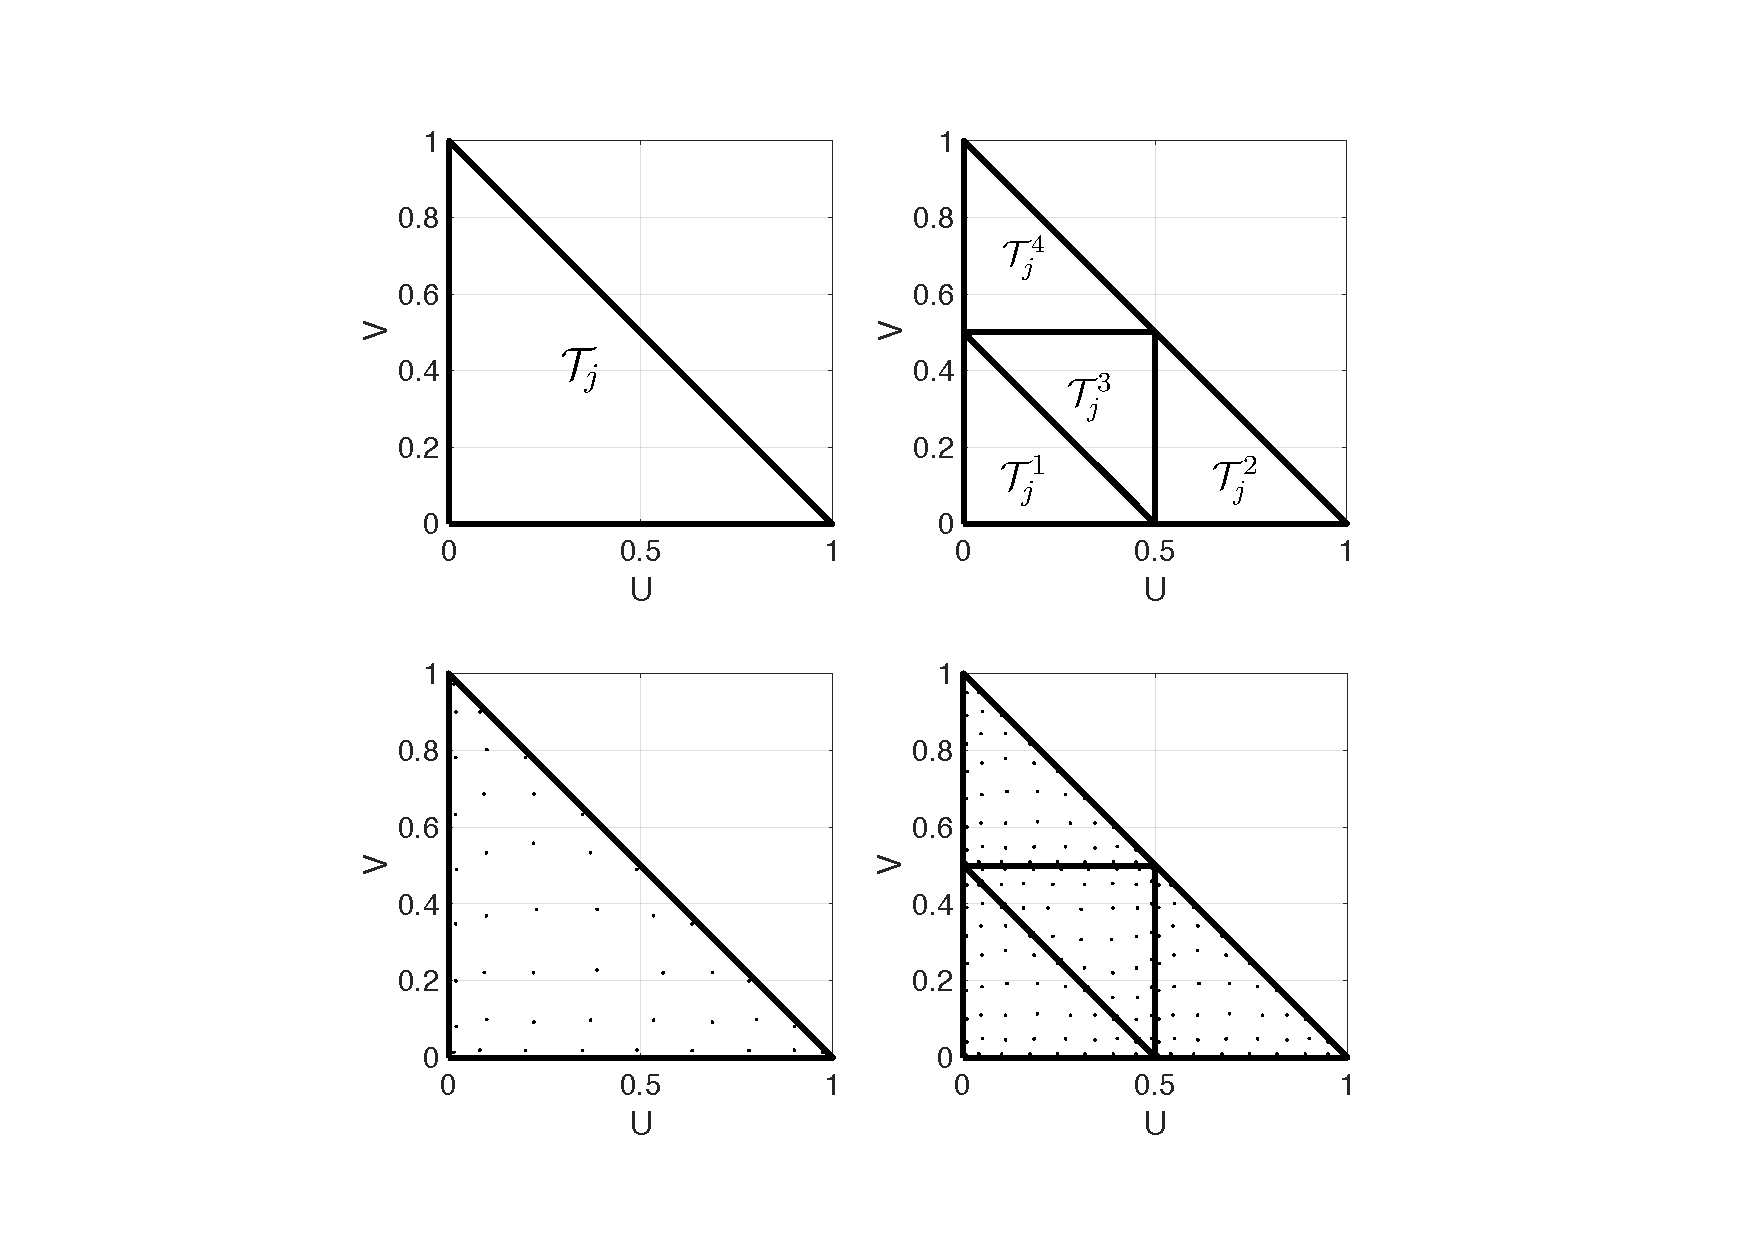
\includegraphics[width=4in]{Triangle_Refine_v2.pdf}
\end{center}
\caption{Description of the refinement process, nested triangles obtained on the canonical triangle and quadrature nodes obtained after refinement}
\label{refinement1}
\end{figure}

Notice that the definition of the surface $\mathcal{S}$ has not changed, as the function $f$ only depends on the skeleton $\mathit{S}$ and the parameter $\sigma$. Notice also that each triangle $\mathcal{T}_j$ has been split into four nested subtriangles $\mathcal{T}_j^1,\mathcal{T}_j^2,\mathcal{T}_j^3,\mathcal{T}_j^4$. See figure \ref{refinement2} and \ref{refinement3}.

\begin{figure}[H]
\begin{center}
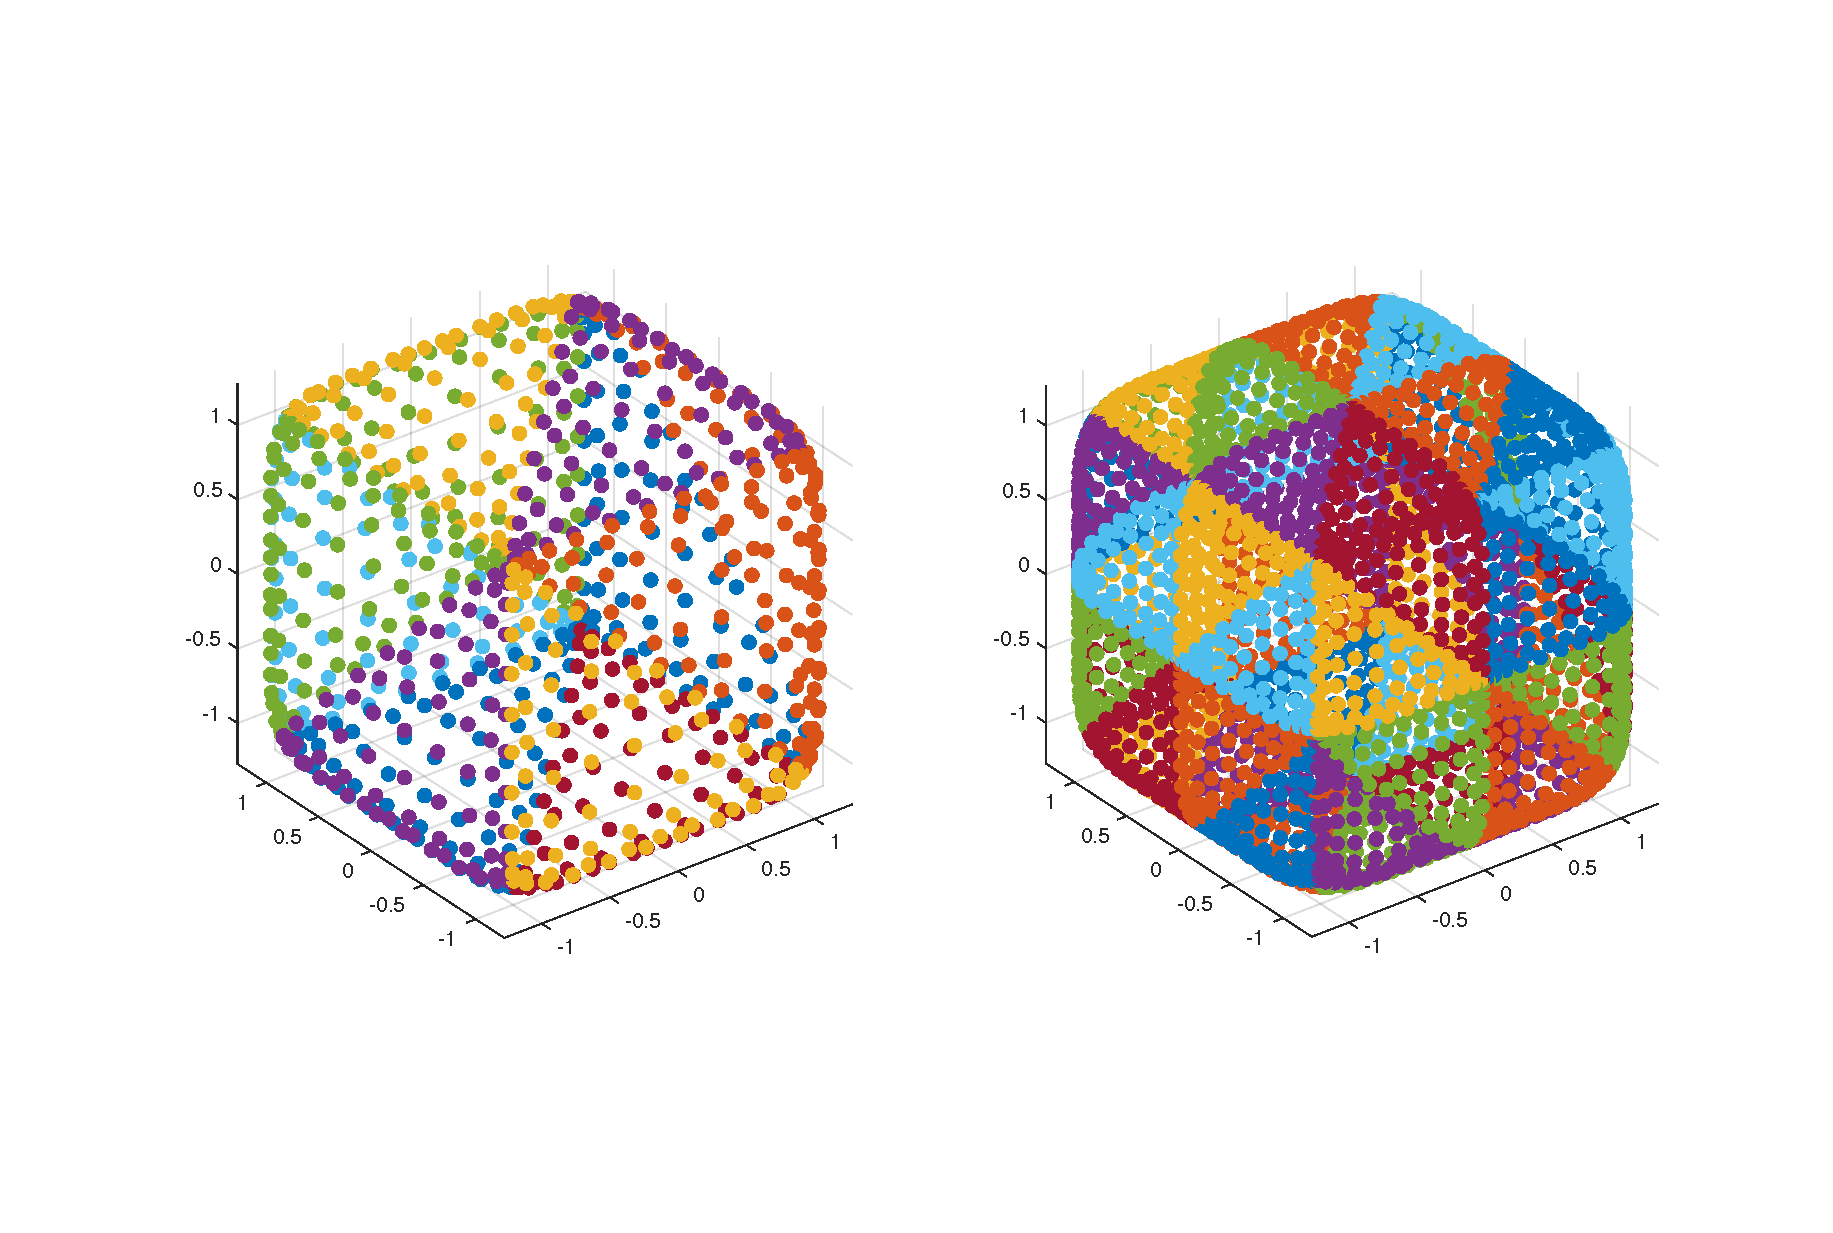
\includegraphics[width=4in]{cloud_points_refinement_v2.pdf}%
\end{center}
\caption{Description of the refinement process, nested triangles obtained}
\label{refinement2}
\end{figure}


\begin{figure}[H]
\begin{center}
\includegraphics[width=4in]{cloud_points_refinement_g2_v2.pdf}%
\end{center}
\caption{Description of the refinement process, nested triangles obtained}
\label{refinement3}
\end{figure}


By doing this we obtain a new atlas with four times more triangles:
$\{\mathcal{T}_j\}_{j=1}^{n_{tri}}\rightarrow
\{\mathcal{T}_j\}_{j=1}^{4\cdot n_{tri}}$ where we can apply the
discretization process of section \ref{disc} and obtain a discretized
surface with four times more points.








\subsection{A Fast Adaptive Algorithm}
\label{sec:fast-adap}


So far we have described how to generate a smooth surface from a closed flat triangulated surface $\mathit{S}$ (skeleton). The degree of smoothness is controled by the parameter $\sigma$. The value of $\sigma$ must be in proportion to the size of the triangles in $\mathit{S}$ (a typical value can be $\frac{1}{5}$ of the size of the triangles). This algorithm requires a regular triangularization of the surface $\mathit{S}$ with triangles of similar size.

In this section we would like to apply this algorithm to geometries with multiscale features. In order to achieve that we need to have a variable degree of smoothness across the surface (dictated by the size of each triangle). That is, if the skeleton has small features in certain region, we need a small $\sigma$ near that region, yet, if the skeleton has at the same time big features in other region, we need a larger $\sigma$ near that region.

In order to achieve that we need to modify the definition of the function $f(\bx)$. The rest of the procedure to build the atlas and the discretization of the charts remains unchanged. Next we define the function $f(\bx)$ for the adaptive case:

\begin{equation}
f(\bx)=\int_{V}\frac{1}{\sigma ^3(\bx)\sqrt{2\pi}^3}e^{-\frac{|\bx-\by|^2}{2\sigma^2(\bx)}}dV_{\by}
\end{equation}
Now we define the surface $\mathcal{S}=\{\bx \mid f(\bx)=\frac{1}{2}\}$.

The function $\sigma(\bx)$ is a $C^{\infty}(\mathbb{R}^3)$ with a value at $\bx$ approximately proportional to the size of the nearest triangle. Next we propose two possibilities (see (\ref{sigma1}) and (\ref{sigma2})):

\begin{equation}\label{sigma1}
\sigma(\bx)=\frac{\sum_{j=1}^{n_{tri}}\sigma_je^{- \frac{|\bx-\bP_j^c|^2}{2\sigma^2_0}}}{\sum_{j=1}^{n_{tri}}e^{-\frac{|\bx-\bP_j^c|^2}{2\sigma^2_0}}}
\end{equation}

Here $\bP_j$ is the center of the $j$'th triangle of the skeleton $\mathit{S}$ and $\sigma_j$ are numbers proportional to the size of the $j$'th triangle of the skeleton. $\sigma_0$ is a parameter provided by the user, typically on the order of the average size of the triangles. Notice that if $\sigma_0\rightarrow \infty$ then $\sigma(\bx)$ is the averaged value of $\sigma_j$; if $\sigma_0\rightarrow 0$ then $\sigma(\bx)$ tend to the value of $\sigma_j$ of the nearest triangle with center at $\bP_j$.

Notice that the expression (\ref{sigma1}) can be computed as a quotient of two Gauss transforms, therefore, a fast algorithm is possible (see [Greengard Fast Gauss Transform]). In this case we are typically in a regime where only the loca interaction is required.

The definition of $\sigma(\bx)$ specified in (\ref{sigma1}) does not achieve perfect adaptivity across a high range of multiscale features. It only achieves some adaptivity across features of the geometry that differ by one order of magnitude in size. If further adaptivity is required (across several orders of magnitude) then we need a more complicated definition of $\sigma(\bx)$ for each fixed value of $\bx$ where we need to evaluate $\sigma(\bx)$ (see \ref{sigma2} and notice that the function $h(z)$ depends also on $\bx$):

\begin{equation}\label{sigma2}
\sigma(\bx)=\frac{\sum_{j=1}^{n_{tri}}\sigma_je^{-\frac{|\bx-\bP_j^c|^2 \lambda^2}{2\sigma^2(\bx)}}}{\sum_{j=1}^{n_{tri}}e^{-\frac{|\bx-\bP_j^c|^2 \lambda^2}{2\sigma^2(\bx)}}}
\end{equation}

Notice that, in this case, we have $\sigma(\bx)$ written in a implicit way. We can consider that $\sigma(\bx)$ is the fixed point of the function $h(z)$ with $z=\sigma(\bx)$, where:

\begin{equation}\label{sigma2}
h(z)=\frac{\sum_{j=1}^{n_{tri}}\sigma_je^{-\frac{|\bx-\bP_j^c|^2 \lambda^2}{2z^2}}}{\sum_{j=1}^{n_{tri}}e^{-\frac{|\bx-\bP_j^c|^2 \lambda^2}{2z^2}}}
\end{equation}

This makes the calculation a bit more complicated, yet we can evaluate it by using an iterative method. To make it more stable we propose to use the relaxation method with $\eta=0.2$ on the first 10 iterations (that is to iterate with $z_{n+1}=\eta h(z_n)+(1-\eta)z_n$) and then use the Newton method for the function $h(z)-z=0$. An appropriate intial guess for $\sigma(\bx)=\sigma_0(\bx)$ is given by the expression \ref{sigma1} with a choice of $\sigma_0$ proportional to the size of the smallest triangle :
 
\begin{equation}\label{sigma0}
\sigma_0(\bx)=\frac{\sum_{j=1}^{n_{tri}}\sigma_je^{- \frac{|\bx-\bP_j^c|^2}{2\sigma^2_1}}}{\sum_{j=1}^{n_{tri}}e^{-\frac{|\bx-\bP_j^c|^2}{2\sigma^2_1}}}
\end{equation}









In the adaptive case, we can still evaluate the function $f(\bx)$ and
$\nabla f(\bx)$ efficiently using the FMM. Next we update the
expressions~\ref{eq:surf} and \ref{surf_nablaf} for the variable
$\sigma(\bx)$ case:

 
\begin{equation}
\begin{aligned}
f(\bx)&=\int_{\mathit{S}}\nabla_{\by}\Big(\frac{\erf\big(\frac{|\by-\bx|}{\sqrt{2}\sigma(\bx)}\big)}{4\pi|\by-\bx|}\Big)\cdot\bn(\by)dS_{\by}=\\
&=\int_{\mathit{S}}\Bigg(\frac{\erf\big(\frac{|\by-\bx|}{\sqrt{2}\sigma(\bx)}\big)}{4\pi|\by-\bx|^3}-\frac{\sqrt{\frac{2}{\pi}}e^{-\frac{|\by-\bx|^2}{2\sigma^2(\bx)}}}{4\pi\sigma(\bx)|\by-\bx|^2}\Bigg)(\by-\bx)\cdot\bn(\by)dS_{\by}
\end{aligned}
\end{equation}

\begin{equation}
\begin{aligned}
\nabla f(\bx)&=\int_{\mathit{S}}\nabla_{\bx}\nabla_{\by}\Big(\frac{\erf\big(\frac{|\by-\bx|}{\sqrt{2}\sigma(\bx)}\big)}{4\pi|\by-\bx|}\Big)\cdot\bn(\by)dS_{\by}=\\
&=\int_{\mathit{S}}-\bn(\by)\Bigg(\frac{\erf\big(\frac{|\by-\bx|}{\sqrt{2}\sigma(\bx)}\big)}{4\pi|\by-\bx|^3}-\frac{\sqrt{\frac{2}{\pi}}e^{-\frac{|\by-\bx|^2}{2\sigma^2(\bx)}}}{4\pi\sigma(\bx)|\by-\bx|^2}\Bigg)dS_{\by}-\\
-&\int_{\mathit{S}} \frac{e^{-\frac{r^2}{2\sigma^2(\bx)}}(\sqrt{2}r^3+\sqrt{2}r\sigma^2(\bx)3)-\sigma^3(\bx)\sqrt{\pi}3\erf{\big(\frac{r}{\sqrt{2}\sigma(\bx)}}\big)}{r^5\sigma(\bx)^3\pi^{3/2}4}(\bx-\by)<(\by-\bx)\cdot \hat{\bn}(\by)>dS_{\by}+\\
+&\int_{\mathit{S}} \frac{e^{-\frac{r^2}{2\sigma^2(\bx)}}}{\sigma^4(\bx)\pi^(3/2)2\sqrt{2}}<(\by-\bx)\cdot \hat{\bn}(\by)>\nabla_{\bx}\sigma(\bx)dS_{\by}
\end{aligned}
\end{equation}

%\begin{equation}
%-\frac{e^{-\frac{r^2}{2\sigma^2}}(\sqrt{2}r^3+\sqrt{2}r\sigma^23)-\sigma^3\sqrt{\pi}3\erf{\big(\frac{r}{\sqrt{2}\sigma}}\big)}{r^5\sigma^3\pi^{3/2}4}
%\end{equation}
In this case we can also use the FMM to speed up this calculation.






\section{Conclusions}




























\bibliographystyle{unsrt}
\bibliography{master}

  
\end{document}  